\let\textcircled=\pgftextcircled
\chapter{Design \& Implementation}
\label{chap:des_imp}

\initial{T}his chapter will discuss in detail the design decisions made in this project, and any specifics of the implementation phase. 
The whole process of the application could be divided into several stages and described using the figure \ref{fig:workflow}. The tweets are taken from Twitter using Twitter API, after which they are passed through two models: a sentiment analysis model and a topic modelling model. Two questions are asked: ``Is a tweet positive or negative?'' and ``Does the tweet talk about a certain topic?''. If at least one of the answers is ``No'' then the tweet is discarded. Otherwise it is marked as being relevant.

The project has been written entirely in Python because most of the existing Natural Language Processing tools, especially the NLTK library, are implemented in 

The rest of the chapter will discuss in detail both of the models and the design decisions behind them. 

\begin{figure}
    \centering
    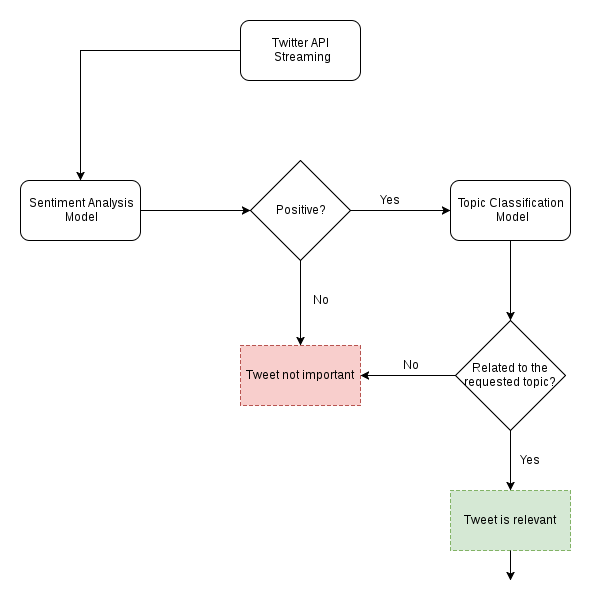
\includegraphics[width=\textwidth]{workflow}
    \caption{General Workflow}
    \label{fig:workflow}
\end{figure}

%=======
\section{Existing Tools}
\label{sec:tools}

The main constraint of this project has been the time limitation. A lot of small steps involved in the processing of data could have been separate study fields, and an immense amount of research could have been potentially devoted to these fields. Because this project is limited in time, for a lot of these cases, only the existing libraries could be used for some techniques. Some of such methods are imperfect and could be improved. This will be discussed in the conclusions chapter in greater detail, but in this chapter it will be mentioned a lot that certain trade-offs had been made to make the project possible. In most cases, existing libraries have been at least tried because, mostly, it is complicated and time-consuming to implement techniques related to Natural Language Processing from scratch, and it also often requires large data sets. 

\paragraph{Twitter API}\mbox{}\\
For the first stage of the project, tweets were obtained from Twitter using Twitter API. The keyword used for search was ``Grangemouth''. Ideally, it would be better to locate tweets geographically and select the ones coming from the Grangemouth area. This would allow to also include tweets that do not mention the area but talk about it. However, as it was discussed in the Context Survey chapter, it is quite complicated to extract the geographical data out of the tweets. Most of them do not contain coordinates, and the heuristics which is widely used in research is not ethical or accurate. This is why it was decided to only focus on the tweets found through search of the ``Grangemouth'' keyword. Streaming of live tweets was also implemented using the same API.

\paragraph{Natural Language Processing Libraries}\mbox{}\\
NLTK\footnote{\url{http://www.nltk.org/}}, the Natural Language Toolkit, is the most well-known platform for Natural Language Processing. It provides access to a variety of methods used to process text and has interfaces which help access some of the largest corpora such as WordNet.

TextBlob\footnote{\url{https://textblob.readthedocs.io/en/dev/}} is a Python library for processing textual data. Although it is often seen as an alternative to NLTK, in come cases it builds on the functionality provided by the NLTK. 

Both of these libraries have been used extensively for different purposes in the project such as noun phrase extraction, text tokenisation, stemming, part-of-speech tagging, parsing, document classification and other. 

Another library used is the preprocessor\footnote{\url{https://github.com/s/preprocessor}}. It is a library for tweet preprocessing in Python and helps extract Twitter-specific entities such as emojis, URLs, and hashtags.

%=======
\section{Sentiment Analysis}
\label{sec:sa}

\subsection{Training datasets}

For sentiment analysis, a large dataset is required to training the statistical model. Creating such a dataset is a hard and time consuming task not only because one would have to go through a large amount of data but also because people do not always agree on the polarity of a sentence. Hence, most of the researchers use several well-known datasets with tagged data. 

In addition, performing sentiment analysis on Twitter data is a specific task, and a model trained on, say, Shakespeare texts could not be used on Twitter data. So, the dataset had to consist of tweets.

Probably, the largest dataset available publicly and referenced on the The World Wide Web Consortium website \footnote{\url{https://www.w3.org/community/sentiment/wiki/Datasets}} is the Thinknook dataset. It consists of 1,578,627 classified tweets, where each tweet is tagged by 0 if it is negative or 1 if it is positive. The advantages of the dataset are, apart from its size, the fact that the data is shuffled within the dataset, so the researcher would not have to put any effort into making sure that when training or testing data is selected from the dataset, approximately half of the tweets are positive and half are negative. However, at the same time, closer look and the first tests showed that, in fact, the dataset consists of the tweets taken from two different sources: Sentiment140 dataset and Kaggle dataset, and the Kaggle dataset only contains tweets about movie reviews, which would make the model biased and not work properly on data related to life in a Scottish town or environmental issues. So, it was decided to only focus on the Sentiment140 dataset.

Sentiment140 dataset \footnote{\url{http://help.sentiment140.com/home}} is one of the most well-known Twitter sentiment analysis datasets and was created by several Stanford University graduates. In the dataset, which is available for access, tweets have several fields and are tagged as positive (4) or negative (0). This dataset, however, is not perfect. For example, the creators say that the data was not labelled manually but automatically. This is usually fine, except, in this case, the authors say that the criteria for automatic tagging has been the smileys: ``we assume that any tweet with positive emoticons, like :), were positive, and tweets with negative emoticons, like :(, were negative'' \cite{sentiment140}. There are several big issues with this approach. First, a smiley can be deceiving or used ironically, as a sarcasm. Secondly, Twitter currently supports emojis, which are complicated Unicode characters, so the heuristics chosen by the researchers would not be efficient. Also, even though roughly half of the tweets in the dataset are positive and half --- negative, the tweets are not shuffled, which means that they had to be shuffled initially and extra care had to be taken to ensure that the training and testing sets had roughly equally spread data in them.

In addition, the same authors also created an online tool that accepts a tweet text request and returns a response with the polarity of the text. Presumably, this tool also uses a model created from the same dataset, so it would make sense to, when validating a newly created model, compare its responses to the ones provided by that model. However, this is impossible because, unlike the dataset, which uses only two possible labels: ``positive'' and ``negative'', the online model adds a third label - ``neutral''. This makes it impossible to compare the two models. 

Unfortunately, the rest of the datasets available would either not be large enough, or not focus specifically on Twitter data, or have other flaws, so the Sentiment140 dataset seemed to be the best one of all the available ones. 

When the main objective is to work with the human-created data, it is not easy to generalise the behaviour of different language models. A model might work well on some data but perform much worse on another data set. That is why throughout this project, the evaluation of the model consisted not only of the statistical evaluation based on testing data but also of manual evaluation based on the `live' data coming directly from Twitter. When creating the model, the main ideas have been based on the results of the most recent research, which has been discussed in the Context Survey chapter, however, in some cases, certain changes have been made due to, for example, better performance of such modified models. Overall, the workflow of the model creation has been following an Expectation-Maximisation process: a model was created, tested, evaluated, and then the loop would start again, with modifications.

\subsection{Feature Vector Extraction}
In order to train a classifier, the input data has to be represented as a feature vector. The success of the entire model depends on the structure of the vector, and it is up to the researcher to design it. In Python, a feature vector is usually a dictionary where the keys are the names of the properties and the values are usually numeric or Boolean values of those properties. For example, it could look like this: \\ \texttt{\{`Length':139, `hasHashtags':True, `containsNegativeWords':False\}}. \\Alternatively, a typical unigram model will look somewhat like this:\\ \texttt{\{`I':True, `am':True, `happy':True, `today':True\}}.\\Note that while in the first case, the vector will always be of the constant size, the latter structure will have a variable number of key-value pairs. Also, since the approaches create a dictionary, which is an unsorted data structure in Python, the order of the words appearing in the input does not matter. Such an approach is called the ``bag-of-words'' approach and is one of the basic feature extraction techniques in Natural Language Processing.  

 A lot of models created for research working with the natural language data use the unigram model \cite{agarwal2011sentiment}. It performs well when the researcher initially does not have a lot of knowledge about the training data, or when it is too vast (like anything concerning natural language) to be summarised in several fields. Also, there is not enough research looking into how different structures of the feature vector affect the performance of the sentiment analysis model and how to best design a feature vector for an input consisting of natural language. It would be interesting to look at this problem, but it is a case for the future studies and does not lie in the scope of this project. In this project, the unigram model is the basis model of the feature vector.  

\paragraph{Tokenisation}\mbox{}\\
The first step of feature extraction os tokenisation. Tokens are `units' of text that the input string is being split into; they are most often words but could also contain URLs, emojis, hashtags, or other Twitter-specific data. The initial simple manual tokenisation showed that simply tokenising text using NLTK provided default methods would not work particularly well. The figure \ref{fig:manual_tok} shows the pairs of tuples, where the first item is the token, and the second item is a number obtained by adding 1 every time it appeared in a positive tweet or subtracting 1 every time the token appeared in a negative tweet. The figure shows the first and the last twenty items of an entire list. Note that the results are not normalised, since it was a small bit of the initial exploratory analysis, and the goal was simply to see what the data looks like, in general. As it can be seen in figure \ref{fig:manual_tok}, most of the most popular tokens are not words but rather punctuation or the `@' character which most often refers to a mention in Twitter. At the same time, this initial simple analysis showed some really important facts about the dataset which would allow make an educated guess about the data. For example, we can say that the word ``love'' is predominantly used in positive tweets, together with words ``great'' and ``you''. In addition, the `\#' sign is also in the first half of the image, which could mean that, overall, hashtags are more popular in the positive tweets.

Predictably enough, the list of token appearing mostly in negative tweets mentions the words ``work'', ``sad'' and ``miss''. It could be surprising for some (or explained in quite a philosophical manner) that this list also contains the pronoun ``I'' in three different forms. 

\begin{figure}
    \centering
    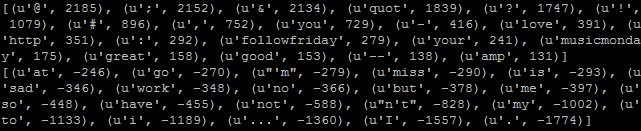
\includegraphics[width=\textwidth]{most_pos_neg}
    \caption{Tokens that appear in most positive and most negative tweets, default tokeniser}
    \label{fig:manual_tok}
\end{figure}

\begin{figure}
    \centering
    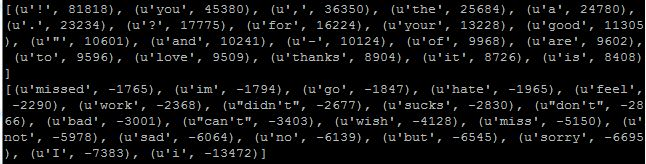
\includegraphics[width=\textwidth]{most_pos_neg_tw_tokenizer}
    \caption{Tokens that appear in most positive and most negative tweets, TweetTokenizer}
    \label{fig:tweettok}
\end{figure}


Thankfully, NLTK also provides a \texttt{TweetTokenizer} which, unlike the default tokeniser, would, for example, see ``@marianna'' as one token and not two different ones. Figure \ref{fig:tweettok} shows the result of the same analysis as in \ref{fig:manual_tok}, but using \texttt{TweetTokenizer}. It can be seen that the list has changed significantly, even though ``I'' and ``i'' are still the tokens that are mostly seen in negative tweets (at this point of the initial analysis, the tokeniser was case-sensitive). 


\paragraph{Pre-processing} \mbox{} \\
Due to the nature of natural language, before any features can be extracted from the input data, it has to be processed. Human-produced data is non-structured, and using the vast amount of unstructured data has been one of the largest problems for data science. Pre-processing data can help make it more structured on later stages of feature extraction. 

Pre-processing natural language input usually involves dealing with such problems as different in upper or lower cases, usage of stop words, abbreviations, any other structures. In the case of this project, it has to be remembered that Twitter has certain structures not normally used in other texts, such as URLs, mentions, hashtags. For the ease of work with different words rather than individual symbols, the pre-processing can be performed immediately after tokenisation. 

For this project, \texttt{ngram\_classifier.NGramClassifier.preprocessing\_extractor()} does all the preprocessing. 

First, the tweet often would have to be decoded. One of the hardest tasks of this project was to keep the data consistent. The data was coming from different sources such as text files of different formats, as well as the live Twitter feed. Some of the input was represented with strings, whereas in other cases it would be in Unicode. The text had to be encoded, and the potential Unicode decode and encode errors had to be accounted for. In some cases, the tweet would not be encoded successfully because it would contain characters that do not exist in English language and could not possibly be translated to ASCII. In cases where no sense could be made out of a tweet, the tweet would have to be skipped. 
\paragraph{}
The \texttt{preprocessor} library was used to extract URLs, mentions, emojis and hashtags from a tweet. For \textbf{URLs}, if there were any in a tweet, they would be each summarised to a single dictionary entry with a `True' value (\texttt{\{``\$URL\$'':True\}}. Most tweets contain at most one external link, so it made sense for the URLs to be summarised to a Boolean value. Deeper research might be able to detect how different links affect the polarity of a tweet. This could potentially be done by accessing the data from the link and trying to determine the polarity of that data, or, alternatively, maybe certain amount of polarity could have been extracted from the domain name itself. However, this is also a case for a further study and is not in the scope of this project. 
\paragraph{}
With the \textbf{mentions}, the situation is not so clear, so the approach taken is just one of a number of possibilities. Similarly to the links, all the mentions are summarised into a dictionary entry of the form \texttt{\{``\$MENTION\$'':True\}}). Alternatively, it was possible to record the number of mentions used in every tweet. However, that number would still be quite low and probably wouldn't affect the resulting model much. Some might argue that it would be useful to use the mention as a source of information about polarity since a mention is a `@' character followed by the username of a user being mentioned, however, it would not be reasonable to assume that each Twitter user is either happy or negative the whole time, even though some people are generally more positive than the others. Overall, this is yet another field of study and is also not in the scope of this project.
\paragraph{}
Unlike the URLs and the mentions, \textbf{hashtags} (`\#' followed by a word or a combination of words that are not separated by any form of whitespace) actually contain text information which could be interpreted in several ways. One of the approaches would be to try and parse the hashtags into the actual text. This would involve quite complicated parsing. Let's look at a sample hashtag, `\#teamGBolympic'. When parsing this hashtag, the desired output would have been the following list: \\ \texttt{[``team'', ``GB'', ``olympic'']}.\\ After that, another bit of processing would have to determine that ``GB'' stands for ``Great Britain''. The result of such parsing would provide data which could be added to the other words and interpreted as additional input for the model. 

On the other hand, it is possible to argue that hashtags are not simply combinations of words. They usually define a concept in a very concise way and are used by a large number of people, becoming trends and being passed between people. If the concept was not trendy and Twitter did not have support for hashtags, the same exact concept could have been expressed in a large number of ways, like almost all concepts in natural language. Yet this specific choice of words and, sometimes, characters, makes hashtags more than words. For that reason, it seemed more sensible to record the hashtag as it is instead of trying to parse it into a list of words. 

\paragraph{}
Finally, the \textbf{emojis} were processed separately. Unlike emoticons, which are simple combinations of text characters, emojis are 12-by-12 pixel images. When received from Twitter as a part from text, they are represented by Unicode sequence of characters. Every emoji has its own unique Unicode codepoint, but the emojis are not sorted in any way which would allow to extract any meaningful information from the code alone. At the same time, each emoji clearly carries a lot of information about sentiment. 

Fortunately, some research has been done to detect the polarity of each emoji. An online ranking exists where each emoji has been given a sentiment score from -1 to 1. The ``Sentiment of Emojis'' paper describes the construction and analysis of the ranking \cite{Kralj2015emojis}. Unfortunately, the ranking only exists as a web page and has no API, so in order to use it, it was necessary to scrape the page. The \texttt{BeautifulSoup} library allows parsing the HTML received from a URL and extract information from the DOM of the page. So, the information from the web page has been scraped and saved locally as a CSV file which contains a list of a format \texttt{"0x1f44f": 0.52}, where the key is the unique codepoint of the emoji and the value is its sentiment score. This allows to avoid scanning the page every time the application is used. If at any point the file cannot be found, the page will be scraped again automatically, otherwise the local file will be used. 

When an emoji is encountered in the tweet, it is looked up in the local file and its sentiment score is extracted. If the emoji is not found (the `vocabulary' of emojis keeps developing), it is being skipped. The sentiment scores of all emojis are summed up into one number and added to the feature vector in the following format: \texttt{"\$EMOJI\$":0.42}. 

\paragraph{}
After all the pre-processing all the URLs, emojis, hashtags and mentions are cut out of the text. The rest of the string is tokenised using \texttt{TweetTokenizer}. All of the tokens are converted to \textbf{lower case}, apart from the cases where the entire word is in upper case. This is just one approach and the could have been done in another way, of course. Usually it is useful to have all the text in one case (say, lowercase), since it, for example, makes ``Today'' (first word in the sentence) be equal to ``today'' (a word in the middle of a sentence) and ultimately improves the statistical model. However, when the data is as informal as it can be on Twitter, it might sometimes be useful to save the case of the words. For example, if the whole sentence is in uppercase, it might mean that the sentence expresses string emotions, and it can help detect polarity of the sentence. 

\paragraph{}
Finally, the resulting list of token is stripped off the so-called \textbf{stop words} and the punctuation. 
The punctuation, however, does not seem to affect the performance of the model at all. Stop words are the non-significant words that, for example, would not be used in a Google query. They act as a glue for the rest of the words in the language. For example, nouns and most adjectives would not be considered stop words, but  articles and conjunctions would be classified as stop words. In a lot of applications related to Natural Language Processing, including sentiment analysis, removing stop words is considered a good practice \cite{poursepanj2013uottawa, kouloumpis2011twitter}. However, experiments showed that the model where the stop words are stripped performs slightly worse comparing to the model where the stop words remained. Research suggests that in some cases, certain stop words are useful for defining sentiment of a text \cite{lin2009joint}. 


\paragraph{Noun Phrase Extraction}\mbox{}\\
Further inquiry into the results of the existing sentiment analysis research opened another topic for discussion. The initial versions of the classifier were working with individual words. However, in natural language, meaning (and, thus, polarity) of individual words often depends on the context. Because of this nature of the natural language, it would be more beneficial to work with phrases rather than individual words. 

Phrase extraction is, however, quite a complicated task since the term ``phrase'' could not be defined formally. In natural language, phrases take different forms, have different lengths and structures. Noun phrase extraction is an important task in Natural Language Processing. The NLTK book \footnote{\url{http://www.nltk.org/book/ch07.html}} describes a way of the noun phrase chunking based on a context-free grammar. The context-free grammar can be defined in a number of ways, and the authors of the book define quite a simple one in the example \footnote{\url{http://www.nltk.org/book/pylisting/code_chunkex.py}}: 
an optional determiner, followed by zero or more adjectives, followed by a noun. 

The grammar looks as follows: 

\texttt{grammar = "NP: {<DT>?<JJ>*<NN>}"}. 

Writing a context-free grammar that would cover all of different forms of noun phrases is a complicated task. In addition, in order to use such a grammar, it is necessary to know the parts of speech of every word. Even though NLTK provides access to large corpora of text, including online chat texts, it is unreasonable to expect every word mentioned on Twitter to be known to NLTK. It would require tagging manually a large amount of text, including abbreviations and slang. In addition, it would require performing error correction on the data because it is unreasonable to expect that the tweets contain to typos or grammatical errors. Overall, it seemed that implementing a noun phrase extractor from scratch could not possibly fit into the scope of the current project.

The TextBlob library provides two methods allowing automatic noun phrase extraction: \texttt{Fast\_NP\_extractor} and \texttt{ConllExtractor}. The second extractor ``uses the CoNLL 2000 corpus to train a tagger'' \footnote{\url{http://textblob.readthedocs.io/en/dev/advanced_usage.html}}. However, neither of the extractors performed on a good level. Both would skip a lot of important noun phrases, find at most one noun phrase in the given tweets, and take around three seconds to extract noun phrases from one tweet. For example, from ``what a lovely day it is right now, going for a walk. I hope to see a lot of sun'' only ``lovely day'' and ``what lovely day'' are being extracted by each of them correspondingly. Even if we assume that the extractor only accepts a sentence at once, both of the extractors still skipped the ``a walk'' phrase.

In a situation where a model has to be trained on tens of thousands of tweets, such poor performance would not be acceptable, and, unfortunately, it was impossible to use noun phrase extraction successfully as a part of this project. 

\paragraph{N-Grams}\mbox{}\\
The existing research and different tests show that using n-grams might give as good results as noun phrase extraction, with much less computation. In fact, some papers on Twitter sentiment analysis mention that unigram model outperforms the bigram or trigram model \cite{agarwal2011sentiment}. Yet, because it seemed counter-intuitive, bigram and trigram models were also tested.

Using NLTK library, it is possible to see the ``most definitive features'' of the model once it is trained. The most definitive bigrams are shown in figure \ref{fig:bigrams}. Each row in this figure shows a feature and how it affects the result given by the classifier. For example, the first row shows that, when the input text contains the combination of tokens ``100'' and  ``followers'', then it makes the tweet positive (``1:0'' shows which label of the two would more likely to be chosen) with the probability 57.2:1.0, which is quite a large proportion. The items in the list are sorted by this proportion, so 57.2 is the largest proportion in the entire sample set.

\begin{figure}
    \centering
    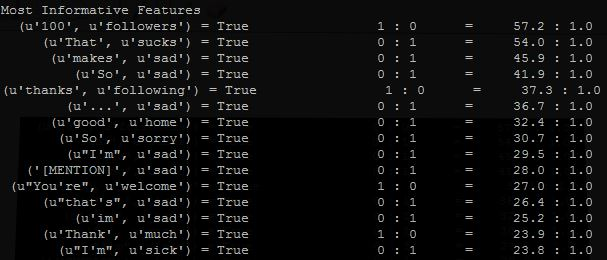
\includegraphics[width=\textwidth]{most_definitive_bigrams}
    \caption{Most definitive bigrams, using Naive Bayes model and TweetTokenizer}
    \label{fig:bigrams}
\end{figure}

The bigram model would, indeed, show slightly lower accuracy than the initial model, where the classifier would use default methods for obtaining unigrams, even though it would still be above 70\% for most of the parameters. However, it was much faster and could be trained on the amount of data that was several times higher than the data that could feasibly be used by the initial model. 

With trigrams, the accuracy dropped to around 60\%, proving the reference made in the paper of Agarwal et. al. that trigrams perform worse than bigrams and unigrams \cite{agarwal2011sentiment}. The model would still be able to train on large amounts of data in a matter of seconds. With Twitter, it could probably be argued that trigrams are too long as constructs to act as meaningful phrases. In a text full of special symbols, mentions, abbreviations, slang and links, and in a text that is also less than 140 characters long, three words will probably have quite a lot of content squeezed into them. Another issue is that removing the so-called ``stop words'' is considered a good technique in sentiment analysis. Stop words are usually short words that do not carry a lot of meaning. When stripped of these words, the text loses its fluency, so the three tokens taken in a row might not even carry any meaning. Another issues is that, statistically, chances of seeing the same trigram several times even in a large dataset are usually quite low, which makes it hard to train a good statistical model.

It is important to note that, for all the experiments with n-grams, NLTK method \\ \texttt{ngrams(input, n)} was used. In accepts the input string and n, which defines how many tokens there are going to be in one n-gram. An n-gram is a tuple of length n. For example, when \texttt{n = 2}, the output list would have items of a format \texttt{("alpha", "beta")}, which is quite predictable. When \texttt{n = 1}, the method still outputs a list of tuples, even though each tuple will only contain one element and, if printed out, will have a format \texttt{("alpha",)} (by putting the comma after the only element, Python specifies that it is, in fact, a tuple). 

When the \texttt{ngrams()} method was used to obtain unigrams, surprisingly enough, the resulting model training was also much faster and memory-efficient than when the default methods were used initially. It could probably be explained by the inefficiency of the NLTK library methods splitting the input. So, this unigram model was used for all the consequent experiments with different classifiers. 

\subsection{Classifiers}
Since the classifiers have already been implemented in the NLTK, it provided an opportunity to test the behaviour of the same dataset on different classifiers and compare them, with minimal effort and time. 
\paragraph{TextBlob polarity} \mbox{}\\
The first model that has been tried for the sentiment analysis was the TextBlob's sentiment analysis model which can be accessed using the \texttt{polarity()} method, which returns -1 if the text is negative and 1 if it is classified as positive. It is an example of a knowledge-based classifier. The results given by the classifier were not very high. When tested on the Sentiment140 dataset, the accuracy of the classifier was 60.04\%. When working with live untagged data, it could be clearly seen that, in a lot of cases, the model would disagree with a general human opinion. The rest of the models created and tested are statistical. 

\paragraph{Naive Bayes Classifier}\mbox{}\\
In most of the papers used as a basis for this project and referenced in the Context Survey, Naive Bayes classifier is mentioned as a very simple classifier that is rarely expected to perform well due to the independence assumptions made, but also as a classifier that often performs almost as good as the state-of-art classifiers.

Indeed, the initial model proved to be quite successful. At different stages of the project, its accuracy would be between 53\% and 88\%.

The initial versions of the classifier were very slow to train. In these versions, a classifier would accept a tweet as a string and use default methods to tokenise the tweet and perform some pre-processing on the input data, such as removing punctuation. 

Figure \ref{fig:nb4000_twtok} shows the most definitive features of a model trained on 4000 tweets, where each tweet was tokenised using \texttt{TweetTokenizer}.  

\begin{figure}
    \centering
    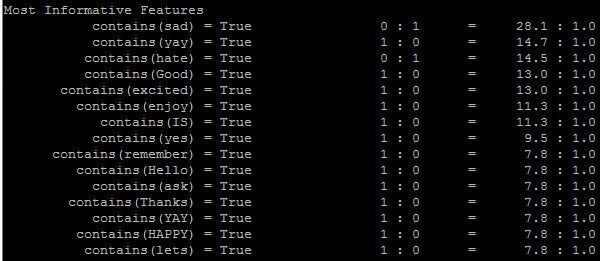
\includegraphics[width=\textwidth]{NB4000_tw_tokenizer}
    \caption{Most definitive feature of a Naive Bayes Model, using TweetTokenizer}
    \label{fig:nb4000_twtok}
\end{figure}

Later the default methods of obtaining feature vectors were replaced by more efficient methods which perform tokenisation and extracting unigrams from the list of tokens.

\paragraph{Support Vector Machine}\mbox{}\\
The Support Vector Machine instance is based on the \texttt{LinearSVC} implementation by the \texttt{sklearn} library. 
Ultimately it was the fastest one to train and the most precise one on terms of the results. The model would accept a large number of tweets as a training set. Empirically, the training size of 300 000 tweets was found to be the best for the purpose of training this sentiment analysis model. The model is used later throughout the project.

\paragraph{Other classifiers}\mbox{}\\
The other two classifiers available in the NLTK library are the Maximum Entropy Classifier and the Decision Tree Classifier.

Unlike the Naive Bayes model, the Maximum Entropy model does not make the independence assumption. From all the models that fit the training data, the Maximum Entropy approach selects the one which has the largest entropy. Intuitively, the model should perform well on the tasks involving Natural Language Processing. However, its current implementation in NLTK did not produce good results. The model was too slow during training and was not memory-efficient (would constantly cause the program to run out of memory). At the same time, the existing SVM and Naive Bayes classifiers performed on a high enough level, so it was decided not to use the Maximum Entropy model. Finally, the results received from that model were significantly lower than the ones returned by the previous models. With 6000 tweets as a training set, the final accuracy was 63\%, which was lower than the Naive Bayes Model or the Support Vector Machine. 

The Decision Tree classifier was the slowest yet. The execution time of training a model on just 1800 tweets exceeded twelve minutes and even though it produced a high accuracy of 80\%, the result was comparable to the one produced by the previous faster models, so it was decided not to use it either.

\paragraph{Resulting platform}\mbox{}\\
The resulting application that performs the sentiment analysis training can be seen as a platform. The main method accepts a number of parameters such as the name of the classifier to use, how many items there should be in an n-gram, the length of training and testing sets, and the name of the feature extractor, because several test ones were written throughout the project. The program can train four different classifiers on custom-defined training and testing data, use three different feature extractors (a simple n-gram extractor that does almost no pre-processing, a noun phrase extractor that tries extracting noun phrases using library methods --- rather unsuccessfully --- and the pre-processing extractor, the most developed feature extractor that does all of pre-processing described above and then extracts n-grams ). This allows to create and compare different models, makes the application scalable and maintainable. It could later be used in other Natural Language Processing-related work.

%=======
\section{Topic Modelling}
\label{sec:tm}

For the topic modelling, the Falkirk Council provided a list of concepts they would like to trace. The first step in designing a model is similar to the sentiment model and requires obtaining enough training data. However, unlike the previous case where the training data could be obtained online, the training data for such specific topic as this could not possibly be found online. There was only one way to form training data: to request a certain amount of tweets using Twitter API and to label them manually or in a semi-automatic way. 

However, it was impossible to get any training data for this topic at all. Most of the concepts have never been mentioned in any tweets mentioning Grangemouth, and the ones that were mentioned did not have enough occurrences to form a plausible training set. 

In addition, Twitter API has certain limits on both number and age of tweets that could possibly be requested \footnote{\url{https://dev.twitter.com/rest/public/rate-limits}}. Currently, the search function allows to make  requests per time window bounded by 15 minutes through the user authentication and 450 requests for the same time window through the application authentication. For this project, application authentication was used. However, there is also a time limit for the tweets that could be requested. Twitter API only allows to request tweets from last several days (the exact number of days has been changing frequently throughout Twitter history). Due to the low Twitter activity around the Grangemouth area and the fact that the tweets mention environmental issues quite rarely, none of the relevant tweets could have possibly gotten into the required time window. Hence, the training data could not have possibly been obtained.

\subsection{Rule-Based Model}
As discussed in the Context Survey, most of the existing topic modelling techniques are based on statistical models, and, hence, all of them require labelled data, even when it comes to unsupervised learning techniques. Thus, none of them could have been used for this task. 

At this point it was clear that any model created could not be possibly made scientifically sound. Introducing sample training data would require a lot of time and effort. However, the biggest problem with this approach is that it would have been impossible to introduce data that would have been purely ``natural'' and not biased, even if the data was created in the process of a user study. 

Therefore, it was decided to create a small manual filter for the given topic which would work with a decent accuracy and could be showed to the client and then change the topic in order to keep the scientific side of this project sound. 

The so-called rule-based model is contained in the \texttt{src/rb\_environmental\_classifier.py} file. The pre-processing methods used in this module was later re-used in the creation of a statistical model. The main approach to this classifier was taken from ``VADER: A Parsimonious Rule-based Model for Sentiment Analysis of Social Media Text'', a paper on sentiment analysis which also used a rule-based approach and claimed that the resulting model outperformed the most common sentiment analysis models \cite{hutto2014vader}. Hutto, the author of the paper, also provides implementation of the classifier\footnote{\url{https://github.com/cjhutto/vaderSentiment}}. 

\paragraph{VADER}\mbox{}\\
The VADER tool is based on the generalizable rules which were created and validated using qualitative
and quantitative methods. The implementation uses constants such as booster word coefficient increase \texttt{B\_INCR = 0.293} and an ALLCAPs increase \texttt{C\_INCR = 0.733}. In every such case, the number is said to have been obtained empirically. The tool uses a list of punctuation, a pre-defined list of negations, some of which are not just the usual negations such as ``couldn't'' but also the less obvious options such as ``uh-uh''. The authors also used a list of degree adverbs, but it was never specified where the list was taken from, and it can be clearly seen that the list only contains a small part of all the degree modifiers used in the English language. Finally, a local vocabulary is also used, which contains words together with their individual sentiment scores.

The processing the VADER uses is based on a single coefficient that is increased or decreased depending on the appearance of different features. First, sentiment score is extracted for every word or emoticon and stored in a list. Then, every word is checked for ALLCAPs and, if the it is written in all uppercase letters, the valence for that word is increased by \texttt{C\_INCR = 0.733}. Similar slight modifications happen for cases such as negation, idioms, and others. Finally, the list of individual scores is summed up and, in case of special punctuation appearing in the input, ``amplified''. The resulting score is then returned.

\paragraph{Grangemouth topic classifier}\mbox{}\\
The Grangemouth rule-based classifier tried to follow the same approach, however, it was clear from the beginning that it would not be very successful. In the case of VADER, the rules --- of the format \texttt{ condition -> modify(coefficient)} --- were carefully designed using both qualitative and quantitative methods. All of these methods require an immense amount of time and need users to label statements manually. Such project could not possibly fit as a part of this project, hence all the coefficients, constants and rules are based on what seemed to be common sense, but obviously none of them were based on scientific results. 

The classifier uses the given list of keywords provided by the Falkirk Council as well as some other pre-defined lists such as a list of mentions which could be relevant to environmental issues. For example, the user names of the Falkirk Council Twitter account (falkirkcouncil), the INEOS and BP Twitter user names. The latter two companies have a number of accounts each all starting with ``INEOS\_'' or ``BP\_'', so regular expressions were constructed for these cases. Also names of the companies were added as well, because some users might not know that the companies have presence on Twitter, and SEPA (Scottish Environment Protection Agency) was included, too. Another list was constructed for anti-mentions since the initial analysis of typical tweets mentioning Grangemouth showed that some accounts will almost exclusively specialise in one topic. For example, \texttt{MadrasRugby} mentions Grangemouth in a lot of its tweets, however, the account only ever talks about rugby.

Overall, the \textbf{initial lexicon} was defined as a collection of groups of words of different parts of speech (e.g. nouns, adjectives). 

As the first step, the lexicon is initialised for the classifier. In order to do that, the program goes through the initial lexicon and, for every word, performs the following:
\begin{enumerate}
    \item The word is \textbf{stemmed} using the \texttt{WordNetLemmatizer} provided by \texttt{NLTK}. Stemming involves removing any morphemes of a word that are not in the core of a word. For example the word ``unbelievable'' should return ``believe'' as a stem. Stemming allows to recognise groups of words regardless of their form. For example, we would usually want to recognise words ``burn'' and ``burning'' as one without having to store both words in the vocabulary and without having to generate all possible forms of the same word since every stem can be involved in the creation of quite a large list of words. Hence, it seemed reasonable to store stems rather than full words. One could argue that other morphemes also carry some amount of information, however, they are not useful when it comes to topic modelling. For example, the form ``cats'' has an affix `-s' which carries a meaning of plurality, however, it does not change the topic itself. So does the suffix `over-' in the word ``overachiever''. When expressed in terms of the First-Order Logic, it can be seen that the affixes provide the functions rather than the arguments. Hence, for the purpose of topic modelling, stems are sufficient sources of information about meaning.
    \item Stem is added to a list of stems of the derived lexicon.
    \item Synonyms of the word are found using the \texttt{wordnet.synsets(word)} function. Potentially, the word network could be grown further by finding synonyms of every synonym. Every synonym is then also stemmed, and the new stems are also added to the dictionary. 
\end{enumerate}
\paragraph{}
At this point the lexicon is considered finalised, and the classification can begin. Again, the classifier works with a single number which is modified slightly depending on appearance of different features in a tweet. The amount of change is a guess based on the knowledge of the data and the fact that all the tweets about Grangemouth going back to as far as 2009 were read.
The classification procedure follows the following approach:
\begin{enumerate}
    \item First, the input is checked for special characters. A horizontal ellipsis is mostly used in tweets containing links, which are mostly news tweets. Currency symbols are usually used in economical news and almost never is complaints about environment. Hence, both types of special character reduce the coefficient.
    \item The tweet is parsed using the \texttt{preprocessor} library. URLs generally reduce the chance that a tweet talks about environment, especially if they are not links to Instagram or Twitter internal links (usually link posts together). All the links on Twitter are currently shortened with the \texttt{t.co} domain, however it is possible to extract the actual URL using \texttt{urllib2} library. Seeing a name mentioned in names or mentions increased the coefficient, whereas seeing a name from the ``anti-mention'' list decreases it.
    \item The tweet is stripped off URLs and mentions.
    \item The tweet is tokenized using \texttt{TweetTokenizer}. Every token is stemmed and the stem is then looked up in the dictionary. Known stems increase the coefficient.
    \item The tweet is checked for idioms. Some tweets have been seen mentioning expressions ``smell a rat'' and ``under fire'' (for example, ``the plan to start fracking is under fire''). The words ``smell'' and ``fire'' are in the list of the initial keywords provided by the Falkirk Council, so the classifier is biased when it notices the words. Hence, when these expressions appear in the tweet, the coefficient is decreased. 
\end{enumerate}

A positive coefficient means that the tweet does, indeed, talk about environmental issues. 
\paragraph{}
Since this was a rule-based approach and none of the data was labelled, the only way to test a model was to do it manually. Several examples were copied from the existing Twitter history and some more examples were hand-written. The only result that could possibly be given by such not precise evaluation is that the classifier seemed to perform reasonably well. The model gave no false negatives and several false positives. At this point it was decided that the result was good enough to show to the client, and the topic was changed.

\subsection{SVM Topic Model}

\paragraph{Topic Selection}\mbox{}\\
A new topic that was supposed to be chosen for the model had to satisfy the following criteria:
\begin{itemize}
    \item It had to have enough accessible samples to train a model.
    \item The topic had to be a sub-topic of a larger topic such that the larger topic was represented by a set of tweets roughly twice as large as the set represented by the sub-topic. 
\end{itemize}
As a result, the larger topic was chosen to be ``Elections'' and the sub-topic was chosen to be ``UK General Elections 2017''. At the time when the topic was chosen, the UK General Election had just been announced. At the same time, when searching for the keyword ``election'', the search also returned a lot of tweets about the investigations concerning the US Presidential Election, the at that time upcoming French Election as well as some other elections in other countries and organisations.

The tweets were collected and saved in a JSON file (\texttt{resources/election\_tweets.txt}) as a list of entries of the following format: \texttt{\{"text": "What should the world expect if Marine Le Pen takes power? https://t.co/ZLRufRmkDW", "label": 0\}}. The `label' value is 1 if the tweets is related to the UK General Election of 2017 and 0 otherwise. The tweets were labelled manually. There are 870 tweets in the dataset, out of which 405 are positive and 465 are negative.

\paragraph{Vocabulary}\mbox{}\\
In order to create a successful model, instead of using simply a bag-of-words approach, it seemed to make sense to use an approach that is a little more complicated. Twitter API does not let access tweets that are older than several days. In addition, Twitter search by keyword returns every tweet containing that keyword, among which are also retweets, re-postings of the original tweets starting with an ``RT'' sign, if requested via the Twitter API. When it comes to popular topics and popular accounts, some tweets become `viral' and get retweeted thousands of times within a time frame of just several hours. This makes the sample of tweets obtained from the Twitter API biased because it might focus on smaller topics that become very popular for a short amount of time and would bias the classifier in the long run.

So, in order to avoid creating this bias, it was necessary to create a basic vocabulary similar to the one provided by the Falkirk Council for the initial task. It was important to generate a vocabulary that would not introduce bias itself. One of the proposed approaches was to generate the dictionary from the news article tags taken from most popular newspapers available in the United Kingdom. Article tagging helps create hierarchy for the publishers, thus introducing opportunities for additional automatic tools such as filtering of search results. Article tagging can, in fact, be an example of a task involving topic modelling, since today the largest publishers who have a large amount of new material published every day do it automatically. For example, Nieman Lab published an article in 2015 that described how New York Times uses machine learning to achieve that goal \cite{niemanlab}.

However, there is no tool that would allow to grow such a network of tags automatically and extract it from a publisher's website. In addition, the tags observed on different websites were too ambiguous and there were simply not enough of them to start a dictionary. For example, figure \ref{fig:guardianTags} shows how Guardian\footnote{\url{https://www.theguardian.com/uk}} tags its articles. The network obtained from it would be quite small and only mostly mention the names of parties and people involved. The figure \ref{fig:indyTags} shows the same problem with the tags used on the Independent website\footnote{\url{http://www.independent.co.uk/}}.

\begin{figure}[ht]

\includegraphics[width=\textwidth]{guardianTags}
\caption{Topics of an article on Guardian}
\label{fig:guardianTags}
\end{figure}

\begin{figure}[ht]
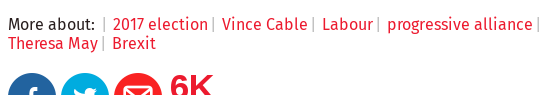
\includegraphics[width=\textwidth]{indyTags}
\caption{Topics of an article on Independent}
\label{fig:indyTags}
\end{figure}

Because of this, it was decided to look into other tools that would help grow the network.

\paragraph{Google Tools}\mbox{}\\
Some of the products created by Google are not well known but can be extremely useful when it is necessary to process immense amount of data. Three Google products provide functionality that allows to extract networks of related words, with different contexts and fir different reasons.

First such tool is Google AdWords \footnote{\url{https://adwords.google.com/}}, which allows creating advertisements and promoting them through the Google platform. As a part of the functionality provided by platform, Google offers to create a set of keywords that would be associated with the advertisement. Figure \ref{fig:googleads} shows the keywords found for ``general election'' combination. 

\begin{figure}[ht]
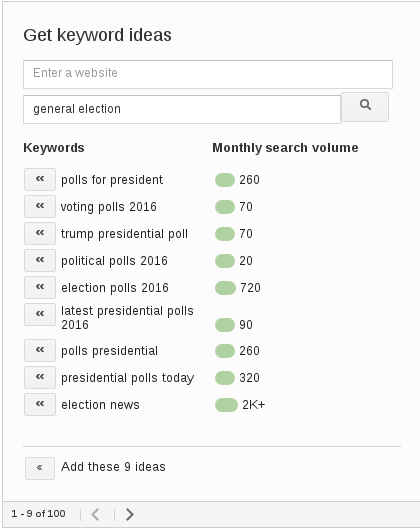
\includegraphics[width=0.7\textwidth]{googleads}
\caption{Related keywords from GoogleAdWords}
\label{fig:googleads}
\end{figure}

As it can be seen, most of the keywords are not relevant to the 2017 UK General Election specifically, and the list is too small to operate on.

Another Google-provided tool that focuses on finding related keywords is Google Correlate\footnote{\url{https://www.google.com/trends/correlate}}. The tool searches through the search patterns of people from the specific period of time and detects common patterns. Figure \ref{fig:googlecorrelation} shows the searches correlated with ``UK general election''. It can be seen that this result is also not perfect despite being far better than the one obtained from GoogleAdWords. The first two results are simply combinations of words from the request, and four other results are different forms of the same word. At the same time, the correlation with one party was found, and with one UK region, too.

\begin{figure}[ht]
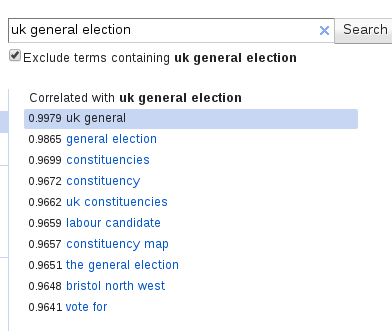
\includegraphics[width=0.7\textwidth]{googlecorrelation}
\caption{Related keywords from Google Correlate}
\label{fig:googlecorrelation}
\end{figure}

Finally, the tool that returned the best results for the initial vocabulary was Google Trends\footnote{\url{https://trends.google.co.uk/trends/}}. Google Trends is a tool that also processes the searches to detect trends and is, in fact, at the core of the Google Correlate. The tool started as a mechanism to create a flu surveillance system based on the symptoms searched on Google by people at different locations. Now the tool provides similar functionality of detecting different trends about any topic requested by the user. When ``2017 UK general election'' was requested, the tool provided useful and interesting data summary including two sections which were later used as a basis for the initial vocabulary. The two sections are Related Topics and Related Queries, two lists of up to 25 entries. A list of related topics provides a list of topics that users searching for the original query (in our case, 2017 UK General Election) search for, too. The second list, related queries, is a list of unprocessed queries that people who search for the original topic search for, too. Both of these lists could be exported as CSV files. Additionally, the network could be grown by expanding topics exported in the Related Topics list.

After all the necessary CSV files had been saved, they could be used in the topic model. First, however, the dictionary had to be finalised. The \texttt{src/vocab\_creator.py} deals with this. First, the CSV files are all read in and a common list of concepts is then written out to one CSV file. This file is the first draft of the vocabulary. Then the vocabulary was modified manually: names of some leaders of the existing UK parties were added, for example. In addition, names, nicknames and Twitter account names were added for every existing UK party. 

After the initial version of the vocabulary has been finalised, it could be expanded in the same way as it was done for the rule-based classifier: by adding stemming the existing words and adding stems of their synonyms.

\paragraph{The Support Vector Machine}\mbox{}\\
As it was discussed in the Context Survey, most of the existing topic classifiers use the usual machine learning techniques including the Support Vector Machine approach and Naive Bayes classification. For this project, it was decided to use the SVM approach. 

There were four feature vectors attempted:
\begin{enumerate}
    \item The first extractor summarises the tweet into a vector of a small size and that looks like this: \texttt{\{`titles': 1, `names': 1, `nouns': 2, `stems': 3, `abbreviations': 2,\\ `mentions': 1\}}. The extractor uses all of the pre-processing described for the rule-based classifier. Its main advantage is that is allows the vector to be very compact. At the same time, it throws away all the information that does not fall into any of the known categories. 
    \item This extractor does not throw away the unknown words. Instead, it adds them to the feature vector with a True Boolean value: \texttt{\{`unknown': True\}}. This allows the SVM to learn more about the text itself, however, might also introduce bias and makes the vector much less compact. Overall, it is hybrid approach which uses a combination of human-defined categories and the Bag of Words approach.
    \item The third extractor is very similar to the second one, except it also combines names and mentions into one category instead of two. This model produces almost the same results as the second feature extractor.
    \item Finally, the fourth extractor is based purely on the Bag of Words approach. This extractor does not need the vocabulary at all and only learns from words seen before. 
\end{enumerate}

After that, k-fold validation was performed on the existing model, for all feature extractors. The results show that the models produce very similar results and it will be discussed in more details in the next section.

\section{Analysis of Results}
\label{sec:analysis}

The models can be evaluated both separately and together. Let's start with the sentiment analysis model.

The platform created allows for easy comparison of different models. The results of the SVM and Naive Bayes models for unigrams, bigrams and trigrams and for training sets of different sizes were obtained using 10-fold validation. For each model, we were interested in both accuracy and recall, since the combination of both describes a model best, and the best model will produce high results in terms of both accuracy and recall.

The model was trained using sets of different sizes: 20000 tweets, 50000, 75000, 100000, 200000 and 300000 tweets.  After the series of experiments was run, the \texttt{matplotlib} library was used to plot the results on a graph.

Figure \ref{fig:nbacc} shows accuracy results obtained in a series of experiments. The model based on unigrams performs best throughout the series. It also plateaus faster than the models based on bigrams and trigrams, but the difference in accuracy is also quite high. 

\begin{figure}[ht]
    \centering
    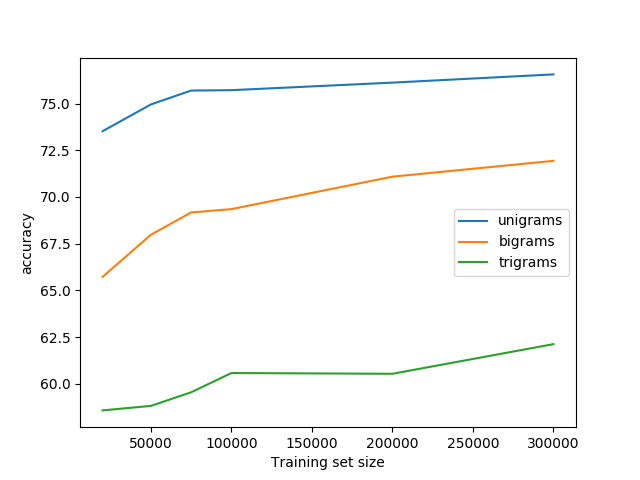
\includegraphics[width=0.8\textwidth]{NaiveBayesacc}
    \caption{Accuracy of Naive Bayes model}
    \label{fig:nbacc}
\end{figure}

Figure \ref{fig:nbrec} shows that, for trigrams, the recall is the highest. On average, the recall for trigrams is about 5\% higher than for bigrams and unigrams. The recall for unigrams and bigrams is similar for unigrams and bigrams, however, unigrams perform slightly better in almost all cases apart from the smallest training set.

Overall, it would be safe to say that the unigrams perform best of all the other architectures. Even though the recall is best for trigrams, the results for trigrams are also quite inconsistent and it falls when the dataset is large.

\begin{figure}[ht]
    \centering
    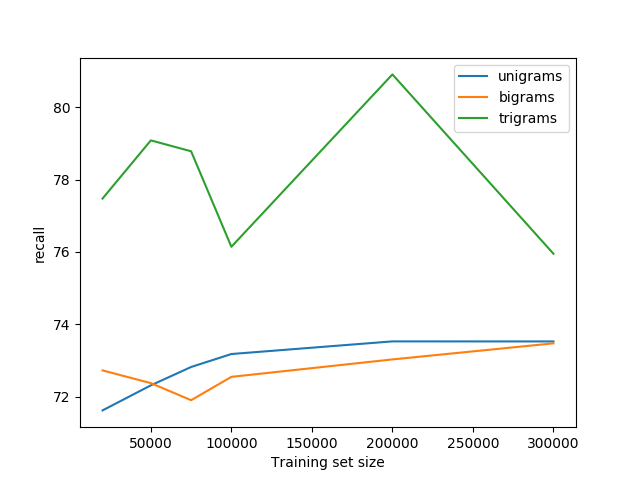
\includegraphics[width=0.8\textwidth]{NaiveBayesrec}
    \caption{Recall of Naive Bayes model}
    \label{fig:nbrec}
\end{figure}

Figure \ref{fig:svmacc} shows the accuracy analysis for the SVM model. In the cae of this model, unigrams perform best, too, and the figure \ref{fig:svmrec} shows that its recall is also better than for any other models. Another thing that could be noticed is that the values for accuracy and recall are pretty similar and that also recall grows as the accuracy grows. 

\begin{figure}[ht]
    \centering
    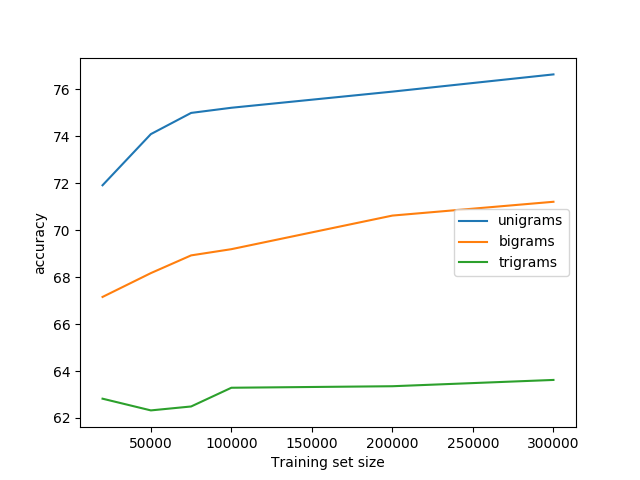
\includegraphics[width=0.8\textwidth]{SVMacc}
    \caption{Accuracy of SVM model}
    \label{fig:svmacc}
\end{figure}

\begin{figure}[ht]
    \centering
    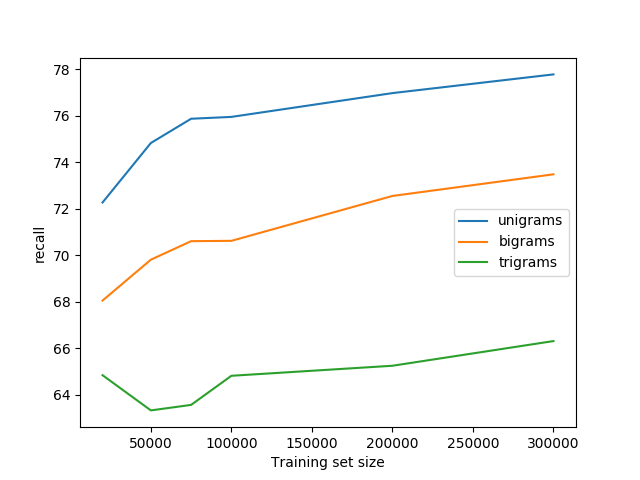
\includegraphics[width=0.8\textwidth]{SVMrec}
    \caption{Recall of SVM model}
    \label{fig:svmrec}
\end{figure}

Figures \ref{fig:acccomp} and \ref{fig:reccomp} compare unigram-based SVM and Naive Bayes models in terms of their accuracy and recall. The accuracy comparison shows that, for smaller datasets, Naive Bayes performs slightly better. The difference between the models is below 2\%. For the largest tested dataset consisting of 300000 tweets, the SVM model performs better than the Naive Bayes. Another interesting fact that could be noticed is that neither of the models could be seen plateauing, so the accuracy is likely to grow even more for larger training sets.

The recall comparison shows that SVM is performs better than Naive Bayes, especially when it is trained using the largest training set. The recall for the SVM is just below 78\%, whereas the same property for the Naive Bayes model is just above 73\%. Moreover, it can be seen that the Naive Bayes model plateaus and might be prone to over-fitting if a larger dataset is used.

\begin{figure}[ht]
    \centering
    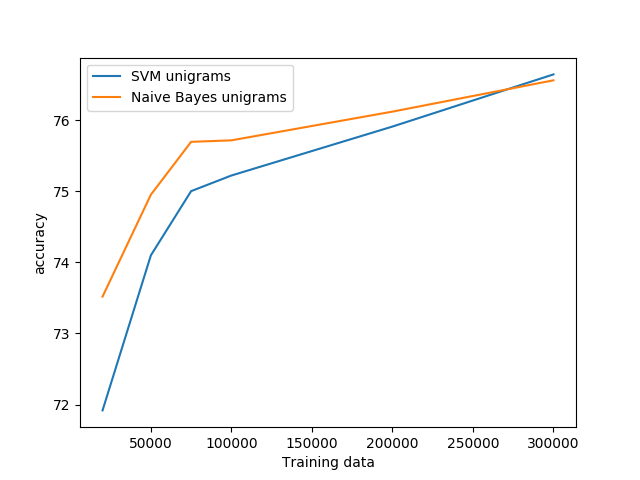
\includegraphics[width=0.8\textwidth]{classACCComp}
    \caption{Comparison of accuracy results}
    \label{fig:acccomp}
\end{figure}

\begin{figure}[ht]
    \centering
    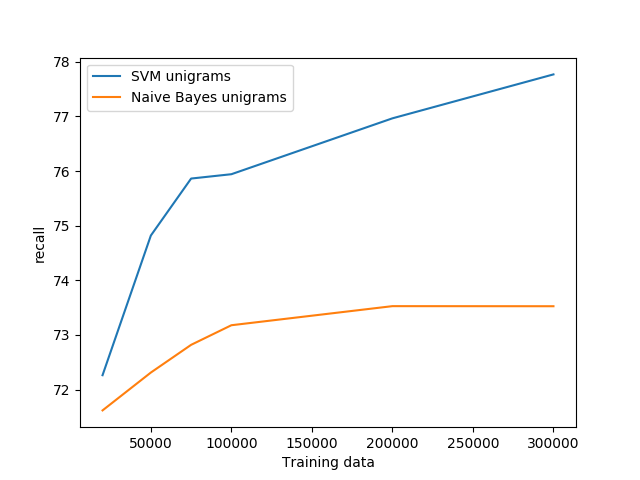
\includegraphics[width=0.8\textwidth]{classRECComp}
    \caption{Comparison of recall results}
    \label{fig:reccomp}
\end{figure}

Overall, it can be concluded that the unigram-based SVM performs the best sentiment analysis. 

Next, it is useful to talk about the topic model. In this case, the dataset was initially quite small (less than 900 tweets) since it had to be labelled manually. In this case, we can compare the performance of the models based on four different feature extractors. 
The first extractor summarised the data into a small dictionary which mentioned several word categories and the number of occurrences of words in a tweet. The second extractor also used the Bag Of Words approach for words that did not fall into any of the categories above. The third extractor also combined the mentions ans names into one category. The final, fourth extractor, only uses the Bag of Words approach and does not consult the vocabulary at any point.

\begin{figure}[ht]
    \centering
    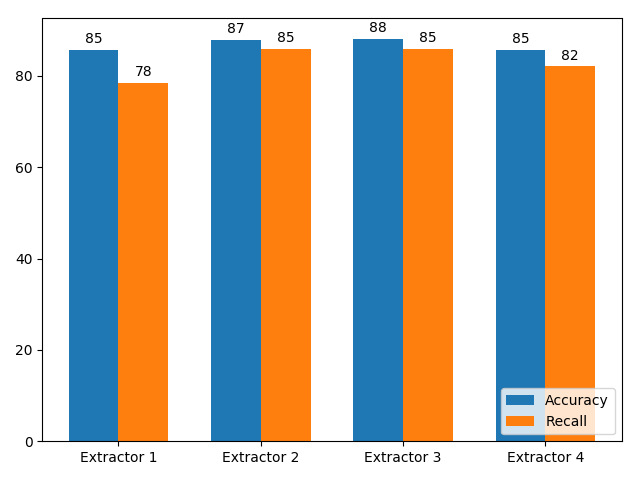
\includegraphics[width=0.8\textwidth]{topic}
    \caption{Comparison of feature extractors of the topic model}
    \label{fig:topicm}
\end{figure}

Figure \ref{fig:topicm} shows the results for different extractors. One important result here is that the extractors using the Bag of Word approach in addition to the human-defined categories --- extractors 2 and 3 ---  perform better than the one using only categories. This shows that humans might not, in fact, be very good at identifying important features which help classify text. The first extractor was based on few intuitive human-created categories. In theory, a text talks about elections if it mentions words from the defined vocabulary and mentions people and parties specified in the vocabulary as well. In reality, the fact that the Bag of Words approach works better means that it is very hard to create a perfect vocabulary. The given vocabulary is not a perfect one and maybe does not mention some of the words which would help in the classification. However, in addition to that, a possible reason Bag of Words approach performs better could be that the words that are not directly related to elections might also carry additional meaning which, combined together in a certain pattern, also helps classify text correctly. Identifying such patterns is quite hard and adding them to the vocabulary is quite complicated, too, because they should not be treated on the same scale as the main words in the vocabulary. For example, a phrase ``promised to'' might theoretically be related to the elections and increase the chances of a tweet being about the UK general elections. However, adding it to the same list as the main words such as ``Brexit'' and ``snap election'' would bias the vocabulary. Instead, it might then be useful to determine the `weight' of every word in the vocabulary. This, however, is hard to calculate manually. This means that the Bag of Words approach has an advantage when used with existing Machine Learning Techniques.

At the same time, extractor 4, which is only based on the Bag Of Words approach, performs worse than the extractors 2 and 3. This means that the categories do help the model perform better, and knowing the structure and main features of the data given helps classify the unseen data.

Of the extractors 2 and 3, the one where the Twitter mentions and names are combined into one category performs slightly better. The difference in the accuracy and recall is very small, but so is the difference in the feature vectors. This difference, again, means that sometimes it is hard to come up with meaningful categories by hand. The tweets usually do not use a lot of mentions or names in one tweet. This means that usually most of them will have values 0 or 1 for either of the categories. Combining the categories into one means that instead of having two small numbers, there is one larger number (usually up to 4). This changes the shape of the feature vector and, hence, changes the results of the model.

Overall, the best topic model is a hybrid one, one based on the combination of human-defined categories for an existing lexicon and the Bag of Words approach. The accuracy for this model obtained using 10-fold validation is 88\% and the recall is 85\%. 
